\documentclass[conference]{IEEEtran}
\IEEEoverridecommandlockouts

% ===== Encoding and language =====
\usepackage[utf8]{inputenc}
\usepackage[T1]{fontenc}
\usepackage[english]{babel}

% ===== Packages =====
\usepackage{cite}
\usepackage{amsmath,amssymb,amsfonts}
\usepackage{algorithmic}
\usepackage{graphicx}
\usepackage{textcomp}
\usepackage{xcolor}
\usepackage{fancyhdr}

% ===== Avoid breaking words with a hyphen at the end of a line =====
% Disables automatic hyphenation; the text remains justified.
\hyphenpenalty=10000
\exhyphenpenalty=10000
\tolerance=2000
\emergencystretch=3em

% ===== Alternating page numbers (odd right, even left) =====
\pagestyle{fancy}
\fancyhf{}
% Page number at ~7pt (as in IEEEtran_HOWTO), a bit lower
\newcommand{\pnum}{\raisebox{-6pt}[0pt][0pt]{\normalfont\fontsize{7}{8}\selectfont\thepage}}
\fancyhead[R]{\ifodd\value{page}\pnum\fi}
\fancyhead[L]{\ifodd\value{page}\else\pnum\fi}
\renewcommand{\headrulewidth}{0pt}

% ===== Initial capital letter (IEEEPARstart) in BOLD =====
\def\IEEEPARstartFONTSTYLE{\bfseries}
\def\IEEEPARstartWORDFONTSTYLE{\bfseries}

% ===== Subsection numbering as a single letter (A, B, C) =====
% Prevents the babel/IEEEtran interaction from showing the section prefix
% (e.g. "V-B" or "I-A") in the subsection titles; forces the IEEE
% single-letter format. Applied at the beginning of the document so it
% prevails over any babel redefinition.
\AtBeginDocument{%
  \def\thesubsection{\Alph{subsection}}%
  \def\thesubsectiondis{\Alph{subsection}.}%
}

% ===== TikZ (figure of the mechanism mounted on the finger) =====
\usepackage{tikz}
\usetikzlibrary{arrows.meta,calc,decorations.pathreplacing}

% Mounting parameters of the mechanism figure on the symbolic finger
\newif\ifconfondo
\confondotrue
\newcommand{\dedoimg}{dedo_sin_fondo.png}
\newcommand{\dedoancho}{18.6cm}
\newcommand{\dedox}{14.1}
\newcommand{\dedoy}{2.7}
\newcommand{\mecEsc}{0.72}
\newcommand{\mecAng}{17}
\newcommand{\mecMx}{13.0}
\newcommand{\mecMy}{6.7}

\graphicspath{{figs/}{./}}

\def\BibTeX{{\rm B\kern-.05em{\sc i\kern-.025em b}\kern-.08em
    T\kern-.1667em\lower.7ex\hbox{E}\kern-.125emX}}

\begin{document}

\title{Partial Kinematic Synthesis of a Finger Exoskeleton Mechanism Using Differential Evolution and Genetic Algorithm}

\author{}

\maketitle
\thispagestyle{fancy}

\begin{abstract}
This work uses two optimization techniques, Differential Evolution (DE) and the
Genetic Algorithm (GA), to obtain the \emph{partial} dimensional synthesis of a
finger exoskeleton mechanism, fitting the movement up to the medial phalanx
(distal interphalangeal joint, DIP). The problem is formulated with 16 design
parameters and an objective function based on the weighted Chamfer distance with
respect to 120 motion-capture (MOCAP) points of a fine pinch grasp, taken from
the public hand kinematics database \cite{ref_pizzolato}, to which a penalty for
movement reversals and a term that favors small dimensions are added. The
hyperparameters of both algorithms are tuned symmetrically with the Optuna tool,
using the same seed and the same number of 25 trials per method. Under this
setup, with the same objective function, the same bounds and the same number of
generations, DE reaches a global error of 2.17~mm versus 2.55~mm for the GA and
produces a more compact mechanism (sum of structural links of 347.2~mm against
457.1~mm). The GA, however, obtains a lower error at the DIP joint (1.43~mm
versus 1.53~mm), while DE keeps the advantage in the global error and in the
proximal phalanx (PIP). The results indicate that both techniques are suitable
for this class of dimensional synthesis and that the specific choice must
optimize the trade-off between fitting error and mechanism compactness.
\end{abstract}

\begin{IEEEkeywords}
differential evolution, genetic algorithm, dimensional synthesis, hand
exoskeleton, dimensional optimization, mechanism chain.
\end{IEEEkeywords}

\section{Introduction}
\IEEEPARstart{H}{AND} exoskeletons are robotic assistance and rehabilitation
devices whose function is to accompany or help recover the movement of the
fingers \cite{ref_exo_review}. For the assistance to be comfortable and safe,
the mechanism must faithfully reproduce the natural joint trajectories of the
finger over the whole flexion range; otherwise, unwanted reaction forces appear
at the joints and the device stops being comfortable for the user
\cite{ref_fourbar_nat}. Achieving that tracking depends largely on correctly
choosing the link lengths of the mechanism, a problem known as
\emph{dimensional synthesis} \cite{ref_de_fourbar}.

Dimensional synthesis for path generation is a hard optimization problem: the
solution space contains large regions where the mechanism simply does not
assemble or reverses its motion, and the relation between the link lengths and
the curve described by the mechanism is nonlinear and has many local optima. For
this reason, classical gradient-based methods tend to get trapped in suboptimal
solutions, which motivates the use of population-based metaheuristics such as
Differential Evolution (DE) and Genetic Algorithms (GA), which can traverse the
search space without needing derivative information
\cite{ref_de_fourbar,ref_tlbo}.

Although both optimization techniques are widely used, their effectiveness
depends on the nature of the problem, on how the variables are represented and on
the tuning of the hyperparameters \cite{ref_ga_pso_de,ref_de_vs_ga}. The choice
between one or the other is rarely obvious and almost always requires testing
them on the specific case to be solved.

Dimensional synthesis of linkages for path generation has historically been
addressed with analytical methods and, more recently, with metaheuristics that
avoid the limitations of gradient-based approaches on nonconvex and discontinuous
functions \cite{ref_de_fourbar,ref_tlbo}. Four-bar mechanisms are a recurring
building block both in path synthesis and in finger exoskeletons, due to their
simplicity and their ability to approximate complex coupler curves with few
parameters \cite{ref_fourbar_nat,ref_exo_stephenson}. When several four- and
five-bar stages are chained, the number of variables grows and the search space
becomes strongly multimodal, which makes the use of global optimization
techniques unavoidable.

In the field of hand exoskeletons, several recent works use swarm-based or
evolutionary optimization to tune the dimensions of mechanisms that reproduce the
natural flexion of the fingers \cite{ref_exo_review,ref_exo_stephenson}. The
choice of algorithm, however, is rarely justified empirically on the specific
mechanism. The direct comparison between families of algorithms has also been
studied: in continuous-domain problems, DE and particle swarm optimization tend
to behave more naturally than the GA, which was originally conceived for discrete
representations \cite{ref_ga_pso_de,ref_de_vs_ga}. Nevertheless, the outcome of
the comparison depends on the encoding, on the operators and on the tuning of
hyperparameters, so it remains necessary to characterize the behavior on real
instances \cite{ref_de_survey,ref_de_sade}.

Unlike those works, here the same formulation, objective function and number of
generations are fixed for both algorithms on a real exoskeleton mechanism, and
not only the fitting error is evaluated but also the coherence and compactness of
the resulting mechanism, two aspects that are decisive for its later manufacture.

In this work both algorithms are used under equal conditions, that is, starting
from the same formulation, the same objective function and the same number of
generations, so that any difference in the result is due to the algorithm and not
to how the experiment was set up. This with the aim of determining the best
technique to synthesize planar mechanisms.

For the comparison to be reproducible, a \emph{partial} version of the mechanism
is optimized, which generates the movement up to the medial phalanx (PIP joint).
This case is smaller than the full three-phalanx model, but it keeps the
essential difficulties of the problem (the coupling between stages, the assembly
constraints and the need for the movement not to reverse), which makes it
possible to study the effect of the optimization algorithm without the added
complexity of the full model.

\subsection{Contributions}
The contributions of this article are: (i) a formulation of the partial
dimensional synthesis problem with 16 parameters, an objective function based on
the weighted Chamfer distance and feasibility penalties; (ii) a controlled
comparison of DE and GA under identical conditions, which evaluates not only the
fitting error but also the coherence and compactness of the resulting mechanism;
and (iii) an analysis of the reasons why DE keeps a slight advantage in this
continuous-variable problem.


\section{Description of the Exoskeleton Mechanisms}
To the original model \cite{ref_palma} a third four-bar stage is added, in order to correct
tracking problems that it presents at the DIP joint. Since in this work the
partial optimization of the chain is carried out, the third four-bar mechanism is
omitted. The present study focuses on the dimensional optimization of the
resulting mechanism (Figure~\ref{fig:diagrama}).

The device reproduces the flexion of the finger through a chain of coupled stages
driven by a single input crank, which makes it possible to govern all the joints
with a single active degree of freedom. The first stage combines a five-bar
mechanism (links $L_1$, $L_2$, $L_3$, $L_4$ and the ground $B_1$) and a four-bar
one (links $L_4$, $L_5$, $h_{sp}$, $d_{sp}$ and the ground $B_2$; the supports
$h_{sp}$ and $d_{sp}$ form a right triangle whose hypotenuse acts as a single
equivalent link) that transfer the movement from the metacarpophalangeal (MCP)
joint to the proximal phalanx (proximal interphalangeal joint, PIP). The second
stage repeats the five-bar pattern (links $L_5$, $L_3$, $L_6$, $L_7$ and the
ground with length $F_p - 2\,d_{sp}$) plus four-bar (links $L_7$, $L_8$, $c_2$
and the distance from the PIP to $h_{sp}$) to carry the movement from the PIP to
the medial phalanx (DIP joint). The proximal phalanx $F_p$ and the medial phalanx
$F_m$ form the finger line (MCP, PIP and DIP joints), while the chain of links
$L_1$--$L_8$ is placed on the back of the hand. The grounds $B_1$ and $B_2$ are
indicated, as well as the rocker $c_2$, the displacements of the support $h_{sp}$
and $d_{sp}$, and the auxiliary angle $\theta_{aux_{fm}}$ that orients the medial
phalanx with respect to the rocker $c_2$. The revolute joints are drawn as white
circles and the fixed supports with hatching. The model stops at the medial
phalanx; the third four-bar mechanism and the distal phalanx are not part of this
version. The \emph{full} model additionally incorporates a third four-bar stage
that locates the distal phalanx; in this study the simplified model is used,
which analyzes up to the medial phalanx. This choice reduces the instance without
losing the essential difficulties of the problem (stage coupling, assembly
constraints and movement monotonicity).

The lengths of the phalanges are considered fixed and are taken from the
measurements of a real human finger: proximal phalanx $L_{FP}=49$~mm, medial
phalanx $L_{FM}=26$~mm and distal phalanx $L_{FD}=24$~mm (the latter only in the
full model). Given a crank position $\theta_2$, the input of the first stage is
obtained through a gear ratio $r_g$ and an offset $\theta_{\text{off}}$ as
$\theta_1=\theta_2/r_g+\theta_{\text{off}}$. The direct kinematics (reported with
detail in \cite{ref_palma}) sequentially solves the four-bar loops and propagates the positions of the PIP and the DIP
along the whole crank sweep. When a configuration does not assemble, produces
non-finite values or generates a reversal of the medial phalanx (non-monotonicity
of the DIP angle), the pose is marked as infeasible and discarded.
Figure~\ref{fig:exo3d} shows the 3D model of the mechanism before optimizing at
the end of its travel, together with the trajectories described by the PIP and
DIP joints during the full crank sweep. Figure~\ref{fig:diagrama} shows the
simplified exoskeleton mechanism mounted on a symbolic finger. The dimensional
synthesis described in the following sections adjusts these lengths up to the
reported solutions.

\begin{figure}[t]
\centerline{\resizebox{\columnwidth}{!}{%
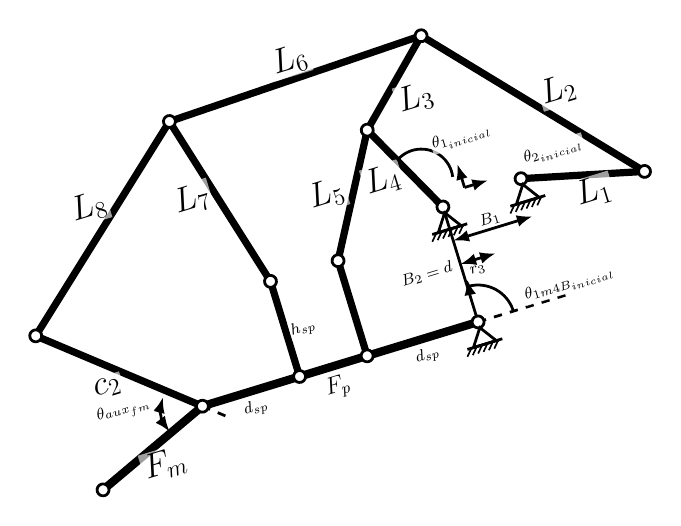
\begin{tikzpicture}[
    x=0.62cm,y=0.62cm,
    esl/.style={line width=2.6pt,line cap=round,black},
    fal/.style={line width=3.0pt,line cap=round,black},
    cota/.style={line width=1.0pt,{Latex[length=2mm]}-{Latex[length=2mm]}},
    dbl/.style={line width=1.0pt,{Latex[length=2mm]}-{Latex[length=2mm]}},
    ref/.style={line width=1.0pt,dashed},
    ejeflecha/.style={line width=1.0pt,-{Latex[length=2mm]}},
  ]
  \ifconfondo
    \node[anchor=center,inner sep=0pt] at (\dedox,\dedoy)
      {\includegraphics[width=\dedoancho]{\dedoimg}};
  \fi
  \begin{scope}[
      shift={($(\mecMx,\mecMy)-(13.7,3.8)$)},
      rotate around={\mecAng:(13.7,3.8)},
      scale around={\mecEsc:(13.7,3.8)},
      transform shape]
  % Node coordinates (chain L1-L8 on the back; fixed phalanges)
  \coordinate (A)  at (1.55, 7.10);
  \coordinate (B)  at (6.97,11.82);
  \coordinate (C)  at (14.53,12.06);
  \coordinate (D)  at (19.48, 6.51);
  \coordinate (E)  at (12.28, 9.94);
  \coordinate (F)  at (13.7, 7.22);
  \coordinate (G)  at (16.06, 7.34);
  \coordinate (H)  at (8.39, 6.63);
  \coordinate (Hf) at (8.39, 3.8);
  \coordinate (I)  at (10.4, 6.63);
  \coordinate (If) at (10.4, 3.8);
  \coordinate (K)  at (5.5, 3.8);
  \coordinate (M)  at (13.7, 3.8);
  \coordinate (Fmp) at (2.1, 2.35);
  % Chain links
  \draw[esl] (G) -- (D);   \draw[esl] (D) -- (C);   \draw[esl] (C) -- (E);
  \draw[esl] (E) -- (F);   \draw[esl] (E) -- (I);   \draw[esl] (B) -- (C);
  \draw[esl] (B) -- (H);   \draw[esl] (A) -- (B);   \draw[esl] (H) -- (Hf);
  \draw[esl] (I) -- (If);  \draw[esl] (A) -- (K);
  \draw[fal] (K) -- (M);   \draw[fal] (K) -- (Fmp);
  \draw[line width=1pt] (F) -- (M);
  % Reference lines
  \draw[ref] (K) -- ($ (A)!1.14!(K) $);
  \draw[ref] (M) -- ++(2.6,0);
  % Joints
  \foreach \n in {A,B,C,D,E,F,G,H,I,K,M,Fmp,Hf,If}{
    \filldraw[fill=white,draw=black,line width=1pt] (\n) circle (0.17);
  }
  % Grounds (fixed supports)
  \foreach \n in {F,G,M}{
    \begin{scope}[shift={(\n)}]
      \draw[line width=1pt] (0,-0.17) -- (-0.34,-0.66) -- (0.34,-0.66) -- cycle;
      \draw[line width=1pt] (-0.52,-0.66) -- (0.52,-0.66);
      \foreach \x in {-0.40,-0.24,-0.08,0.08,0.24,0.40}{
        \draw[line width=0.6pt] (\x,-0.66) -- (\x-0.18,-0.86);
      }
    \end{scope}
  }
  % Labels
  \tikzset{lab/.style={font=\itshape\LARGE, fill=white, fill opacity=0.62,
                       text opacity=1, inner sep=1pt},
           labp/.style={font=\itshape\footnotesize, fill=white, fill opacity=0.7,
                       text opacity=1, inner sep=0.6pt}}
  \node[lab] at ($ (G)!0.5!(D) + (0.15,-0.55) $) {$L_1$};
  \node[lab] at ($ (D)!0.5!(C) + (0.8,0.15) $) {$L_2$};
  \node[lab] at ($ (C)!0.5!(E) + (0.45,-0.6) $) {$L_3$};
  \node[lab] at ($ (B)!0.5!(C) + (0,0.55) $)   {$L_6$};
  \node[lab] at ($ (A)!0.5!(B) + (-0.2,0.7) $) {$L_8$};
  \node[lab] at ($ (B)!0.5!(H) + (-0.75,0.3) $){$L_7$};
  \node[lab] at ($ (E)!0.5!(I) + (-0.7,0.25) $){$L_5$};
  \node[lab] at ($ (E) + (0.0,-1.50) $)      {$L_4$};
  \node[lab] at ($ (A)!0.5!(K) + (-0.45,-0.35) $){$c_2$};
  \node[lab] at ($ (K)!0.5!(Fmp) + (0.2,-0.55) $){$F_m$};
  \node[labp] at ($ (K)!0.5!(Hf) + (0,-0.5) $) {$d_{sp}$};
  \node[labp] at ($ (If)!0.5!(M) + (0,-0.5) $) {$d_{sp}$};
  \node[lab] at ($ (Hf)!0.5!(If) + (-0.05,-0.62) $) {\itshape\large $F_p$};
  \node[labp] at ($ (H)!0.55!(Hf) + (0.5,0) $) {$h_{sp}$};
  \node[labp] at ($ (F)!0.5!(M) + (-1.0,0) $) {$B_2=d$};
  % Dimensions B1 and r3
  \coordinate (b1a) at ($ (F) + (0,-1.0) $);
  \coordinate (b1b) at (G |- b1a);
  \draw[cota] (b1a) -- (b1b);
  \node[labp] at ($ (b1a)!0.5!(b1b) + (0,0.28) $) {$B_1$};
  \coordinate (r3a) at ($ (F) + (0,-1.7) $);
  \coordinate (r3b) at ($ (r3a) + (1.05,0) $);
  \draw[cota] (r3a) -- (r3b);
  \node[labp] at ($ (r3a)!0.5!(r3b) + (-0.1,-0.32) $) {$r_3$};
  % Input angles
  \draw[line width=1pt] ($ (F) + (0.50:0) $) ++(55:0.9) arc (-10:123:0.9);
  \node[labp,anchor=east] at ($ (F) + (2.0,1.75) $) {$\theta_{1_{inicial}}$};
  \draw[ejeflecha] ($ (F)+(0.75,0.35) $) -- ++(0,0.7);
  \draw[ejeflecha] ($ (F)+(0.75,0.35) $) -- ++(0.7,0);
  \node[labp,anchor=west] at ($ (G) + (0.2,0.50) $) {$\theta_{2_{inicial}}$};
  \draw[line width=1pt] ($ (M) + (0:1.05) $) arc (0:88:1.05);
  \draw[ejeflecha] ($ (M) + (88:1.05) $) -- ++(0.02,0.2);
  \node[labp,anchor=west] at ($ (M) + (1.45,0.30) $) {$\theta_{1m4B_{inicial}}$};
  \draw[dbl] ($ (K) + (150:1.15) $) arc (148:200:1.15);
  \node[labp,anchor=west] at ($ (K) + (-3.0,0.55) $) {$\theta_{aux_{fm}}$};
  \end{scope}
\end{tikzpicture}%
}}
\caption{Simplified exoskeleton mechanism mounted on a symbolic finger: the chain
of links $L_1$--$L_8$ is placed on the back of the hand and the phalanges $F_p$
and $F_m$ are aligned with the proximal and medial phalanges of the finger. The
shape of the links corresponds to the mechanism before optimizing.}
\label{fig:diagrama}
\end{figure}

\begin{figure}[t]
\centerline{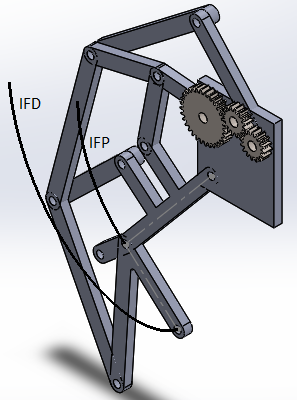
\includegraphics[width=0.55\columnwidth]{exo1.png}}
\caption{3D model of the mechanism before optimizing, at the end of its travel,
with the trajectories followed by the PIP and DIP joints.}
\label{fig:exo3d}
\end{figure}

\section{Formulation of the optimization problem}
\subsection{Design variables}
The design vector $\mathbf{p}\in\mathbb{R}^{16}$ groups the two grounds, the eight
links $L_1$--$L_8$, the rocker $c_2$ of the second four-bar stage, the
displacements of the support $h_{sp}$ and $d_{sp}$, the auxiliary angle of the
medial phalanx $\theta_{aux}^{FM}$, the gear ratio $r_g$ and the input angular
offset $\theta_{\text{off}}$. Table~\ref{tab:bounds} summarizes the search bounds.
The length of each link is bounded to 60~mm at most to favor a compact and
manufacturable mechanism, and the auxiliary angle $\theta_{aux}^{FM}$ is limited
to $70^\circ$ to avoid an anatomically infeasible hyperflexion of the medial
phalanx that would cause mechanical interference with the user's finger.

\begin{table}[htbp]
\caption{Design variables and search bounds}
\begin{center}
\begin{tabular}{|l|c|c|}
\hline
\textbf{Parameter} & \textbf{Min.} & \textbf{Max.} \\
\hline
$B_1$, $B_2$ (mm) & 15 & 60 \\
\hline
$L_1$--$L_8$ (mm)        & 10 & 60 \\
\hline
$c_2$ (mm)      & 10 & 55 \\
\hline
$h_{sp}$ (mm)            & 5 & 30 \\
\hline
$d_{sp}$ (mm)            & 5 & 23 \\
\hline
$\theta_{aux}^{FM}$ (deg) & 0 & 70 \\
\hline
$r_g$ (gear ratio) & 1.0 & 8.0 \\
\hline
$\theta_{\text{off}}$ (rad) & $-\pi$ & $\pi$ \\
\hline
\end{tabular}
\label{tab:bounds}
\end{center}
\end{table}

\subsection{Objective function}
The fit is measured with the symmetric Chamfer distance \cite{ref_chamfer}
between the motion-capture point cloud $M$ and the simulated trajectory $S$. The
set of reference points was obtained from the public database
\cite{ref_pizzolato}. Before evaluating the error, the simulated trajectory is
rigidly aligned (rotation $R$ and translation $\mathbf{t}$) with the data through
a Procrustes solution \cite{ref_procrustes}, so that the error reflects the
\emph{shape} of the curve and not its absolute placement in the plane:
\begin{equation}
d_C(M,S)=\frac{1}{|M|}\!\sum_{\mathbf{m}\in M}\!\min_{\mathbf{s}\in S}\lVert \mathbf{m}-\mathbf{s}\rVert
+\frac{1}{|S|}\!\sum_{\mathbf{s}\in S}\!\min_{\mathbf{m}\in M}\lVert \mathbf{s}-\mathbf{m}\rVert .
\label{eq:chamfer}
\end{equation}
where $M$ is the set of motion-capture (MOCAP) points, $S$ is the set of points
of the simulated trajectory, $\mathbf{m}$ and $\mathbf{s}$ are individual points
of each set. The first term penalizes MOCAP points without a nearby simulated
point and the second penalizes simulated points that move away from the target
curve; their sum is a metric that is robust to sampling differences between the
two curves.

The objective function combines the shape error of the two trajectories (that of
the PIP and that of the DIP), a monotonicity penalty $P_{\text{mono}}$ on the DIP
to avoid movement reversals, and two soft regularization terms that push toward
small dimensions and auxiliary angle without degrading the fit. The term
$P_{\text{mono}}$ penalizes trajectory inversions (hooks or loops) in which the
exoskeleton mechanism moves backward over its path; its inclusion guarantees that
the simulated trajectory progresses monotonically without forming loops that
would cause jamming in the mechanism or unwanted forces on the finger:
\begin{align}
f(\mathbf{p}) =\;& w_{IFP}\,d_C(M_{IFP},S_{IFP}) + w_{IFD}\,d_C(M_{IFD},S_{IFD}) \nonumber\\
& + w_{m}\,P_{\text{mono}}(S_{IFD}) + w_{d}\!\sum_{i}\!L_i + w_{a}\frac{\theta_{aux}^{FM}}{\pi}.
\label{eq:obj}
\end{align}
where $d_C(M_{IFP},S_{IFP})$ and $d_C(M_{IFD},S_{IFD})$ are the Chamfer distances
between the MOCAP points and the simulated trajectory at the PIP and DIP joints
respectively, $P_{\text{mono}}(S_{IFD})$ is the penalty for trajectory inversions
at the DIP, $\sum_{i} L_i$ is the sum of the lengths of the structural links, and
$\theta_{aux}^{FM}$ is the auxiliary angle of the medial phalanx normalized by
$\pi$. The weights are $w_{IFP}=0.40$, $w_{IFD}=0.60$, $w_{m}=5.0$ and
$w_{d}=w_{a}=5\times10^{-4}$. A greater weight is assigned to the DIP because it
is the joint farthest from the input and, therefore, the hardest to fit: it
accumulates the errors of the two stages. The weight values are adjusted through
iterative experimental tests until an adequate balance between the shape error,
the reversal penalty and the regularization is obtained. Infeasible
configurations (without assembly or with reversal) receive a fixed penalty of
$1000$, which creates wide plateaus in the search space and reinforces the
multimodal character of the problem. The formulation, the bounds and the
objective function are identical for DE and GA, so that the comparison measures
the algorithm and not the formulation.

Table~\ref{tab:restricciones} summarizes the kinematic constraints applied during
the evaluation of each individual. If any of these conditions is violated, the
configuration is considered infeasible and receives the fixed penalty of $1000$.

\begin{table}[htbp]
\caption{Kinematic constraints applied in both algorithms}
\begin{center}
\begin{tabular}{|l|l|}
\hline
\textbf{Constraint} & \textbf{Penalty condition} \\
\hline
No assembly & The mechanism does not close in some pose \\
\hline
Non-finite values & NaN or infinity is generated \\
\hline
Medial phalanx reversal & Non-monotonicity of $\theta_{fm} > 0.5^{\circ}$ \\
\hline
Minimum lengths & Some link $\leq 5$~mm \\
\hline
Support geometry & $F_p - 2\,d_{sp} \leq 1$~mm \\
\hline
Out-of-range positions & Some coordinate $> 300$~mm \\
\hline
\end{tabular}
\label{tab:restricciones}
\end{center}
\end{table}

\section{Evaluation of the optimization techniques}
Both algorithms are run with the same random seed (42), a conventional value
widely adopted in previous evolutionary optimization studies that guarantees the
reproducibility of the results, and the same maximum number of generations (300),
a budget validated as sufficient given that DE records its last improvement near
generation 257 and the GA near generation 268, so that both exploit the full
budget without premature stagnation. To avoid the performance depending on
hyperparameters chosen by hand -- in the case of DE: mutation strategy, population
size, mutation factor range and recombination rate; in the case of the GA:
population size, crossover and mutation probabilities, SBX and polynomial
distribution indices, and tournament size -- a common source of bias when
comparing metaheuristics, the hyperparameters of each algorithm are tuned
automatically and symmetrically with Optuna \cite{ref_optuna}, using the
tree-structured Parzen estimator sampler (TPE). The procedure is identical for DE
and the GA: in a first stage, Optuna performs 25 trials per algorithm, the same
number for both, with short runs that evaluate the fitness reached for different
combinations of hyperparameters; in a second stage, the best combination found is
used in a deep run of 300 generations, whose results are the ones reported. The
Optuna search uses the same seed (42) in both cases, so that the tuning is
reproducible and fair. Table~\ref{tab:config} summarizes the resulting
hyperparameters. The reported results were obtained with Python and the libraries
NumPy~2.0.2, SciPy~1.13.1 and Optuna~4.9.0; it is worth warning that the figures
may differ slightly when using other versions of these libraries, since Optuna's
TPE sampler may select different hyperparameters for the same seed and SciPy may
alter the trajectory of the differential evolution, so that the exact
reproduction requires fixing those versions.

\subsection{Differential Evolution}
Differential Evolution is a population-based technique for optimization in
continuous spaces, whose variants and applications have been the subject of
extensive reviews \cite{ref_de_recent,ref_de_image}. In this work the
\texttt{differential\_evolution} implementation of SciPy with the
\texttt{best1bin} strategy is used, which is an open-source library for Python
that implements the differential evolution algorithm for the global optimization
of nonlinear and multimodal functions. The hyperparameters tuned by Optuna are a
relative population size $\text{popsize}=28$, a differential mutation factor that
varies randomly in each generation within the range $[0.54,\,0.85]$ and
recombination $0.77$, with tolerance $10^{-7}$. In each generation, the trial
vectors are built from the best individual and from the scaled difference between
two randomly chosen individuals. This differential mutation automatically scales
its steps with the dispersion of the population: when the population is spread out
the steps are large (exploration) and, as it converges, the steps are reduced
(exploitation), without needing to fix a constant mutation amplitude.

\subsection{Genetic Algorithm}
A real-coded GA is implemented with tournament selection (size 3), simulated
binary crossover (SBX) \cite{ref_sbx} and polynomial mutation. SBX and polynomial
mutation are operators suitable for continuous variables; their distribution
indices, previously set by hand, are here determined by Optuna together with the
rest of the hyperparameters. The hyperparameters tuned by Optuna are a population
of 52 individuals, crossover probability $0.63$, mutation probability $0.22$,
distribution indices $\eta_c=16$ (SBX) and $\eta_m=14$ (polynomial mutation) and
elitism of 2 individuals. An early-stopping criterion by stagnation with a
tolerance of 100 generations without improvement is applied; in the reported run
the GA keeps improving until an advanced phase and exhausts the 300 generations
without triggering that stop, which indicates that Optuna's tuning finds a
configuration that keeps enough genetic diversity to keep exploring the search
space throughout the assigned budget.

\begin{table}[htbp]
\caption{Configuration of the algorithms (hyperparameters tuned with Optuna)}
\begin{center}
\begin{tabular}{|l|l|}
\hline
\textbf{Differential Evolution} & \textbf{Genetic Algorithm} \\
\hline
strategy: best1bin & selection: tournament (3) \\
\hline
popsize: 28 & population: 52 \\
\hline
mutation: $(0.54,0.85)$ & crossover: SBX ($\eta_c=16$) \\
\hline
recombination: 0.77 & mutation: polynomial ($\eta_m=14$) \\
\hline
maxiter: 300 & generations: 300 \\
\hline
tol: $10^{-7}$ & $p_{cx}=0.63$, $p_{mut}=0.22$ \\
\hline
seed: 42 & elite: 2, tolerance: 100 \\
\hline
\multicolumn{2}{|l|}{Tuning: Optuna (TPE), 25 trials per algorithm, seed 42} \\
\hline
\end{tabular}
\label{tab:config}
\end{center}
\end{table}

\section{Results}
\subsection{Fitting error}
Table~\ref{tab:resultados} gathers the metrics of both runs. DE obtains a global
error of 2.17~mm, slightly lower than the 2.55~mm of the GA. The distribution by
joint, illustrated in Figure~\ref{fig:errores}, shows that DE fits the proximal
phalanx better (PIP: 2.82~mm against 3.68~mm), while the GA, once tuned,
reproduces the distal interphalangeal joint with greater fidelity (DIP: 1.43~mm
against 1.53~mm of DE). Overall, the two solutions are very close in shape error,
which confirms that both techniques are able to propagate the movement adequately
up to the end of the mechanism.

\begin{table}[htbp]
\caption{Optimization results (simplified model)}
\begin{center}
\begin{tabular}{|l|c|c|}
\hline
\textbf{Metric} & \textbf{DE} & \textbf{GA} \\
\hline
Global error (mm)      & \textbf{2.1736} & 2.5543 \\
\hline
PIP error (mm)         & \textbf{2.8156} & 3.6813 \\
\hline
DIP error (mm)         & 1.5317 & \textbf{1.4273} \\
\hline
Fitness                & \textbf{0.002335} & 0.002720 \\
\hline
Evaluations (nfev)    & 135\,970 & 15\,052 \\
\hline
$\sum$ structural links (mm) & \textbf{347.2} & 457.1 \\
\hline
\end{tabular}
\label{tab:resultados}
\end{center}
\end{table}

\begin{figure}[htbp]
\centerline{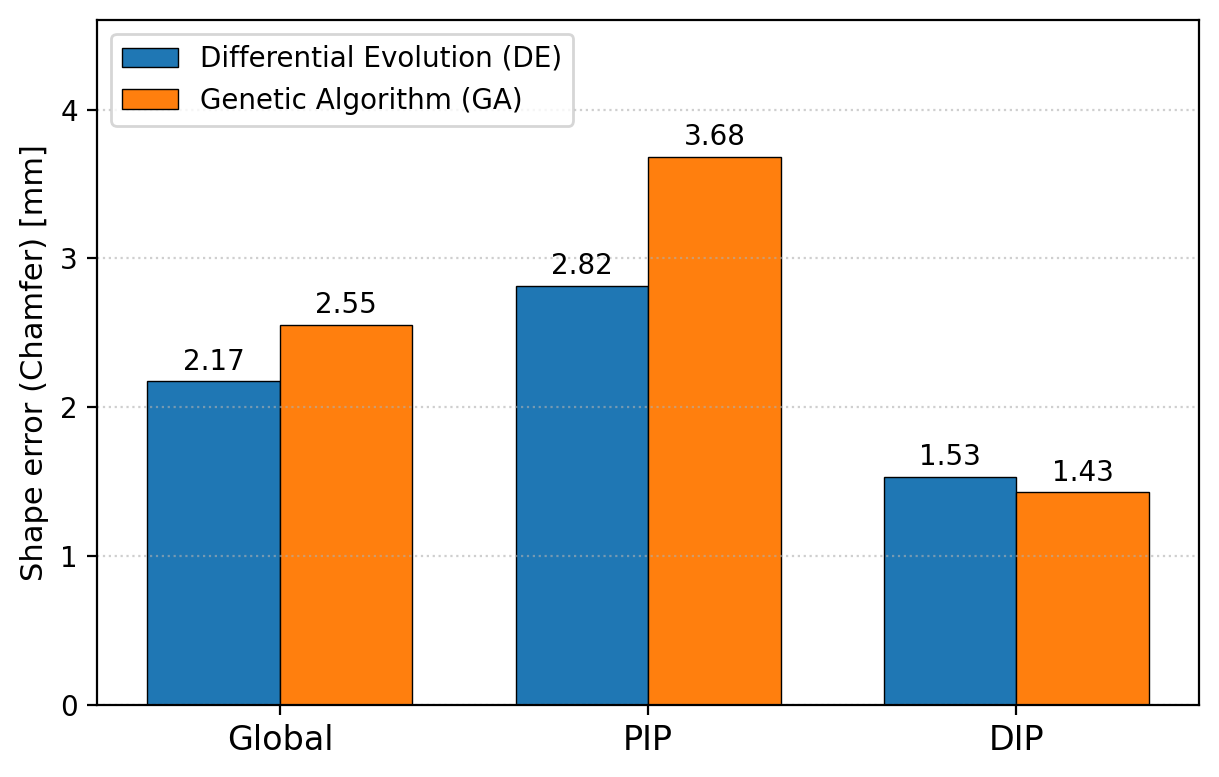
\includegraphics[width=0.92\columnwidth]{comparacion_errores.png}}
\caption{Shape error (Chamfer distance) global, at the PIP and at the DIP for DE
and the GA. DE dominates in the global error and at the PIP, while the GA fits
the DIP slightly better.}
\label{fig:errores}
\end{figure}

\subsection{Dimensional analysis}
Table~\ref{tab:dimensiones} compares, link by link, the dimensions of the
reference CAD design against those optimized by DE and the GA. The lengths
obtained by DE are consistent with the bounds of Table~\ref{tab:bounds} and give
rise to a compact mechanism, where the sum of the eleven structural links ($B_1$,
$B_2$, $L_1$--$L_8$ and $c_2$) is 347.2~mm for DE, 457.1~mm for the GA and
approximately 380.0~mm for the base CAD design. That is, DE not only obtains a
lower global error, but also delivers the most compact mechanism of the three,
while the GA tends toward solutions larger than the reference design itself.
Compactness is desirable for the manufacture, the weight and the portability of
the device on the user's hand, so it constitutes a design criterion as relevant
as the fitting error itself.

\begin{table}[htbp]
\caption{Link dimensions (mm): base CAD design against the optimal solutions of
DE and GA}
\begin{center}
\begin{tabular}{|l|c|c|c|}
\hline
\textbf{Parameter} & \textbf{Base CAD} & \textbf{DE} & \textbf{GA} \\
\hline
$B_1$  & 18.00 & 37.33 & 39.19 \\
\hline
$B_2$  & 20.00 & 39.62 & 59.87 \\
\hline
$L_1$  & 35.00 & 16.00 & 31.84 \\
\hline
$L_2$  & 49.00 & 46.56 & 51.84 \\
\hline
$L_3$  & 25.00 & 16.61 & 33.01 \\
\hline
$L_4$  & 20.00 & 21.60 & 38.83 \\
\hline
$L_5$  & 25.00 & 32.15 & 38.15 \\
\hline
$L_6$  & 55.00 & 39.85 & 51.26 \\
\hline
$L_7$  & 35.00 & 19.16 & 38.22 \\
\hline
$L_8$  & 52.00 & 52.07 & 53.01 \\
\hline
$c_2$  & 46.01 & 26.30 & 21.84 \\
\hline
$h_{sp}$ & 17.00 & 14.91 & 15.63 \\
\hline
$d_{sp}$ & 18.00 & \phantom{0}7.87 & \phantom{0}5.00 \\
\hline
$\sum$ structural & 380.0 & \textbf{347.2} & 457.1 \\
\hline
\end{tabular}
\label{tab:dimensiones}
\end{center}
\end{table}

\subsection{Trajectory biofidelity}
Figure~\ref{fig:biofid} overlays the trajectories simulated by DE and by the GA
on the 120 MOCAP points of the fine pinch grasp, both for the PIP and for the
DIP. Both solutions follow the physiological shape closely: DE reproduces the PIP
and the DIP with Chamfer errors of 2.82~mm and 1.53~mm, while the GA accompanies
them with errors of 3.68~mm (PIP) and 1.43~mm (DIP). The DIP curve of the GA
reproduces the natural flexion with greater fidelity, obtaining 0.10~mm less
error than DE at that joint. Overall, both solutions exhibit a satisfactory
biofidelity: DE offers better global tracking (2.17~mm versus 2.55~mm of the GA)
and at the PIP, while the GA presents a specific advantage at the DIP.

\begin{figure}[htbp]
\centerline{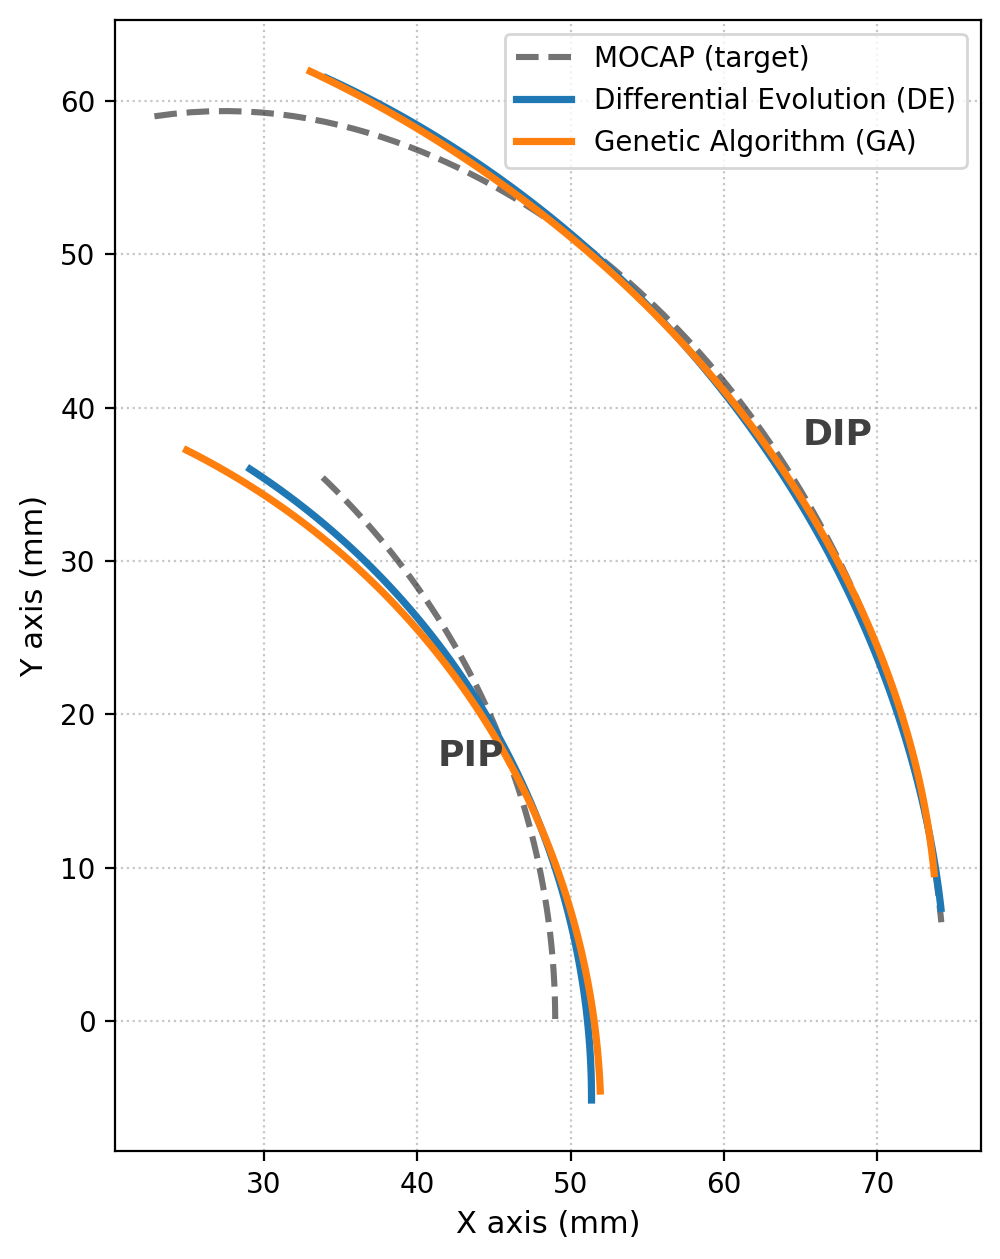
\includegraphics[width=0.85\columnwidth]{biofidelidad_comparacion.png}}
\caption{Trajectory biofidelity: simulated curves of the PIP and the DIP for DE
and the GA, overlaid on the MOCAP points (target) of the fine pinch grasp.}
\label{fig:biofid}
\end{figure}

\subsection{Convergence}
Figure~\ref{fig:convergencia} presents the convergence curves. Both algorithms
descend steadily and use practically the whole number of available generations:
DE records its last improvement near generation 257 and the GA near generation
268, so that neither stagnates early. DE reaches an objective function value of
0.002335, while the GA converges to 0.002720. It is worth noting that the GA
arrives at that result with a considerably smaller number of objective function
evaluations (Table~\ref{tab:resultados}), which reflects its different mechanism
for sampling the search space.

\begin{figure}[htbp]
\centerline{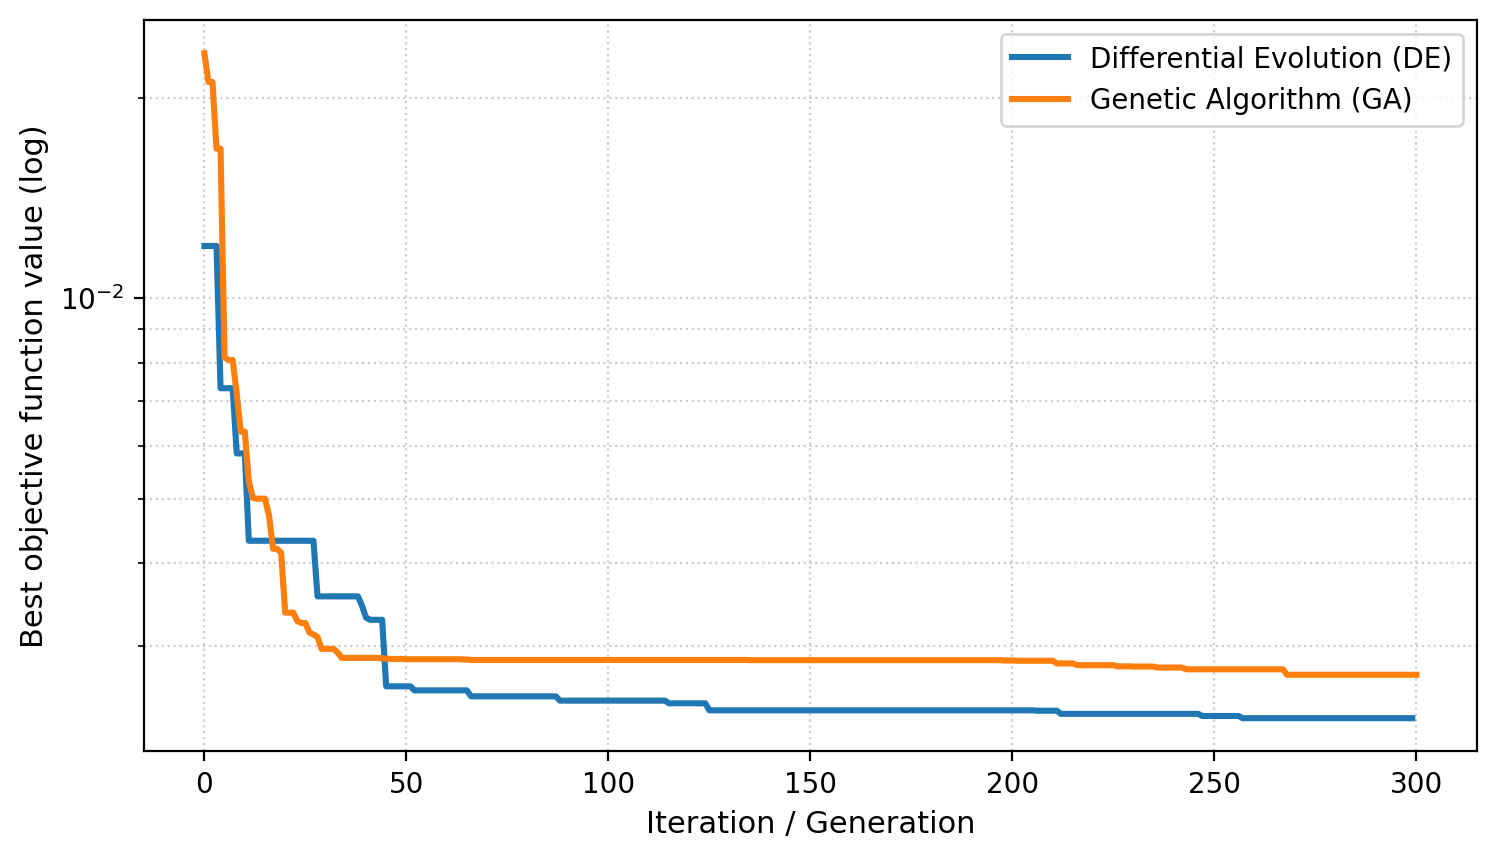
\includegraphics[width=0.92\columnwidth]{comparacion_convergencia.png}}
\caption{Convergence curves of DE and the GA. Both methods descend steadily
during almost all the generations; DE converges to a fitness of 0.002335 and the
GA to 0.002720.}
\label{fig:convergencia}
\end{figure}

\section{Discussion}
The design space of the dimensional synthesis is \emph{continuous} and highly
multimodal, with large infeasible regions (without assembly or with reversal of
the medial phalanx) that generate plateaus in the objective function. The
advantage of DE in this scenario comes from the way it builds each new solution:
instead of applying a fixed step size, it adds to one individual the difference
between two other individuals of the population. Thus, the magnitude of the change
adapts by itself to how spread out the population is: when the individuals are
distributed over the space, the changes are large and the algorithm explores;
when the population concentrates near a good solution, the changes are reduced
automatically and the algorithm refines the fit. This automatic step adjustment,
without needing to fix it in advance, fits naturally with continuous variables
such as the link lengths \cite{ref_de_survey,ref_ga_pso_de} and explains, to a
large extent, that DE reaches a global error of 2.17~mm and, above all, the most
compact mechanism.

The real-coded GA relies on SBX crossover and polynomial mutation. Once its
distribution indices ($\eta_c$, $\eta_m$) and its probabilities are tuned with
Optuna, instead of being set by hand, the GA reaches a global error of 2.55~mm,
very close to that of DE, and even surpasses it at the distal interphalangeal
joint (DIP). This result shows that DE does not systematically dominate GAs in
continuous problems \cite{ref_de_vs_ga,ref_ga_pso_de}: the observed gap is
reduced notably when both algorithms start from a fair tuning. The trade-off of
the GA in this case is that it tends toward larger solutions, which penalizes the
compactness of the mechanism.

It is worth pointing out a methodological limitation regarding computational cost.
DE is evaluated with a vectorized and parallel implementation, while the GA is
run in pure Python; for this reason, the comparison of execution times is biased
and is not reported as a merit criterion. Instead, the \emph{quality of the
solution} and the number of function evaluations (nfev) are emphasized as a fairer
computational metric. DE reaches a slightly lower global error despite performing
more evaluations, while the GA obtains a very close solution with a considerably
smaller number of evaluations, which suggests that each method explores the search
space with a different efficiency.

\section{Conclusion}
The partial dimensional synthesis (up to the medial phalanx) of a finger
exoskeleton mechanism is obtained using the optimization techniques Differential
Evolution and real-coded Genetic Algorithm, under a single formulation, a single
objective function and the same number of generations, and with the
hyperparameters of both methods tuned symmetrically with Optuna (TPE sampler, 25
trials per algorithm). DE obtains a global error of 2.17~mm versus 2.55~mm of the
GA and, notably, delivers the most compact mechanism (347.2~mm of sum of
structural links, against 457.1~mm of the GA). Once tuned, the GA is competitive
and even fits the distal interphalangeal joint (DIP) better. The analysis suggests
that, for this class of continuous and multimodal problems, DE's differential
mutation, which adjusts the size of its steps by itself, offers a slight advantage
in global error and, above all, in compactness, while a well-tuned GA reaches a
comparable fit quality. DE is recommended as a reference method when the
compactness of the mechanism is a priority, without this ruling out the GA as a
valid alternative for this class of dimensional synthesis.

As future work the following is considered: (i) extending the optimization to the
full three-phalanx model, incorporating the distal phalanx and the third four-bar
stage; (ii) carrying out multi-seed comparisons with statistical tests to estimate
the robustness of each algorithm; (iii) implementing both algorithms under equal
computational conditions (same language and same level of vectorization), so that
their execution times can be compared without bias; and (iv) physically validating
the optimal mechanism through prototyping and measurement of the real trajectories.
\begin{thebibliography}{00}

\bibitem{ref_pizzolato} S. Pizzolato, L. Tagliapietra, M. Cognolato,
M. Reggiani, H. M\"uller, and M. Atzori,
``A large calibrated database of hand movements and grasps kinematics,''
\textit{Scientific Data}, vol. 4, 170151, 2017.

\bibitem{ref_exo_review} H. K. Yap, J. H. Lim, F. Nasrallah, and C.-H. Yeow,
``Hand exoskeleton design and human--machine interaction strategies for
rehabilitation: a review,'' \textit{Bioengineering (MDPI)}, vol. 9, no. 11, 682, 2022.

\bibitem{ref_fourbar_nat} M. A. Leal-Naranjo, C. R. Torres-San Miguel, M. Carbajal-Romero, and G. Urriolagoitia-Sosa,
``Design optimization of a four-bar exoskeleton with natural finger
trajectories,'' \textit{Open Engineering}, vol. 13, 20220456, 2023.

\bibitem{ref_de_fourbar} J. A. Cabrera, A. Simon, and M. Prado,
``Optimal synthesis of mechanisms with genetic and differential evolution
algorithms,'' \textit{Mechanism and Machine Theory}, vol. 73, pp. 132--145, 2014.

\bibitem{ref_tlbo} S. Sleesongsom, S. Bureerat, and N. Pholdee,
``Four-bar path generation synthesis using a teaching--learning-based
optimization algorithm,'' \textit{Biomimetics (MDPI)}, vol. 11, no. 3, 160, 2024.

\bibitem{ref_ga_pso_de} M. Varaee and M. R. Ghasemi,
``Comparison of three evolutionary algorithms: GA, PSO, and DE,''
\textit{Industrial Engineering \& Management Systems}, vol. 11, no. 3,
pp. 215--223, 2012.

\bibitem{ref_de_vs_ga} J. Tvrd\'ik,
``Differential evolution versus genetic algorithms in multiobjective
optimization,'' in \textit{Lecture Notes in Computer Science}, Springer, 2006,
pp. 1--10.

\bibitem{ref_exo_stephenson} R. V. Deshmukh and H. Godse,
``Optimal synthesis of the Stephenson-II linkage for a finger exoskeleton using
swarm-based optimization algorithms,'' \textit{Journal of Bionic Engineering},
vol. 20, pp. 1--16, 2023.

\bibitem{ref_de_survey} M. Pant, H. Zaheer, L. Garcia-Hernandez, and A. Abraham,
``Differential evolution: a review of more than two decades of research,''
\textit{Engineering Applications of Artificial Intelligence}, vol. 90, 103479, 2020.

\bibitem{ref_de_sade} A. K. Qin, V. L. Huang, and P. N. Suganthan,
``Differential evolution algorithm with strategy adaptation for global numerical
optimization,'' \textit{IEEE Transactions on Evolutionary Computation},
vol. 13, no. 2, pp. 398--417, 2009.

\bibitem{ref_chamfer} H. G. Barrow, J. M. Tenenbaum, R. C. Bolles, and H. C. Wolf,
``Parametric correspondence and chamfer matching: two new techniques for image matching,''
in \textit{Proc. 5th Int. Joint Conf. Artificial Intelligence (IJCAI)}, 1977, pp. 659--663.

\bibitem{ref_procrustes} J. C. Gower,
``Generalized Procrustes analysis,''
\textit{Psychometrika}, vol. 40, no. 1, pp. 33--51, 1975.

\bibitem{ref_optuna} T. Akiba, S. Sano, T. Yanase, T. Ohta, and M. Koyama,
``Optuna: a next-generation hyperparameter optimization framework,'' in
\textit{Proc. 25th ACM SIGKDD Int. Conf. Knowledge Discovery \& Data Mining
(KDD)}, 2019, pp. 2623--2631.

\bibitem{ref_de_recent} S. Das, S. S. Mullick, and P. N. Suganthan,
``Recent advances in differential evolution -- an updated survey,''
\textit{Swarm and Evolutionary Computation}, vol. 27, pp. 1--30, 2016.

\bibitem{ref_de_image} A. Khellal et al.,
``A comprehensive review on differential evolution and its applications in image
processing,'' \textit{Archives of Computational Methods in Engineering},
vol. 29, pp. 4519--4565, 2022.

\bibitem{ref_sbx} K. Deb and R. B. Agrawal,
``Simulated binary crossover for continuous search space,''
\textit{Complex Systems}, vol. 9, no. 2, pp. 115--148, 1995.

\end{thebibliography}

\end{document}
